\begin{figure*}[tb]
    \begin{subfigure}{0.49\textwidth}
        \centering
        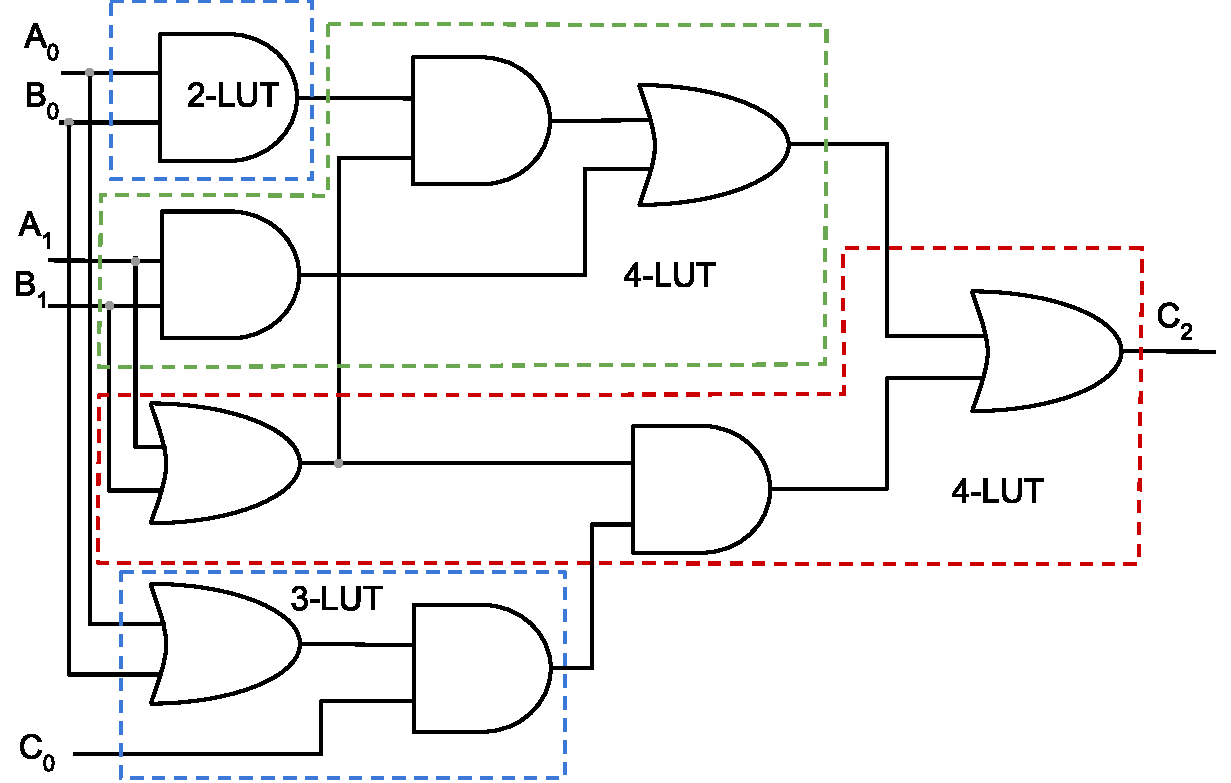
\includegraphics[width=0.92\textwidth]{img/cla_bad.pdf}
        \caption{An implementation that uses four LUTs contains redundancy.}\label{fig:eg:bad}
    \end{subfigure}
    \hfill
    \begin{subfigure}{0.49\textwidth}
        \centering
        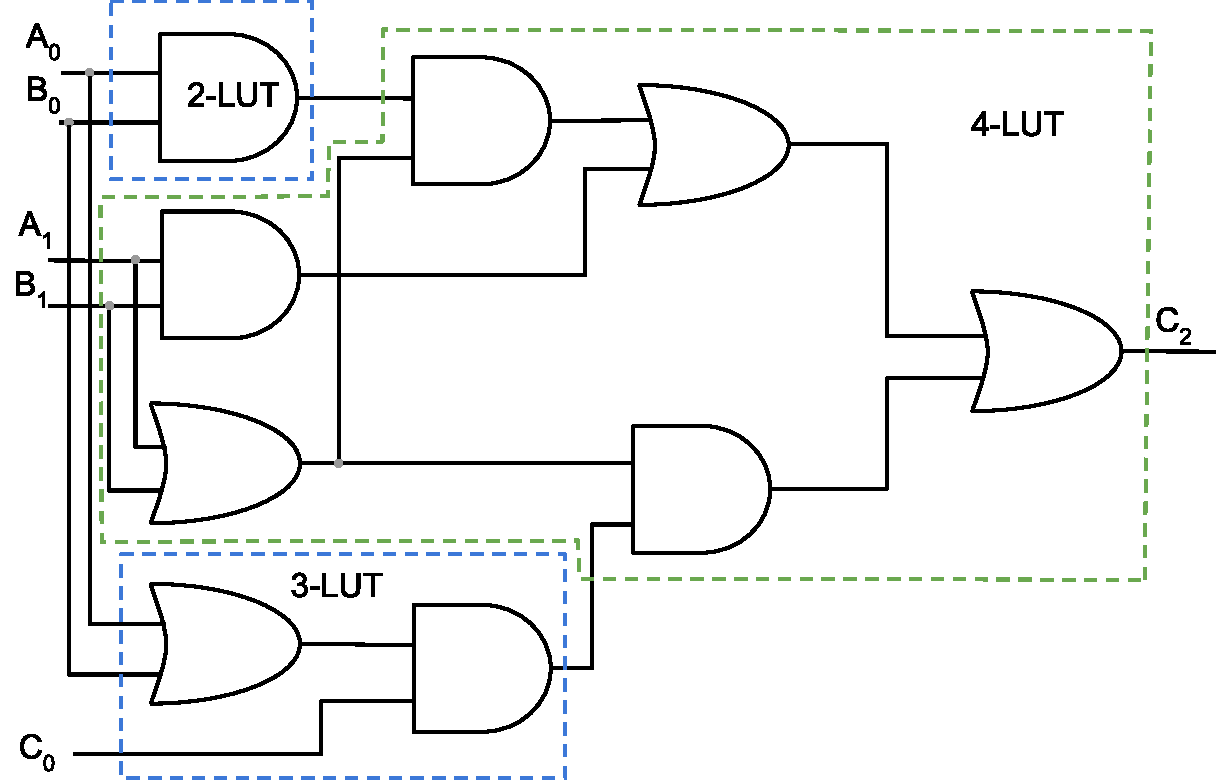
\includegraphics[width=0.92\textwidth]{img/cla_good.pdf}
        \caption{The sink cut of logic can expand its cover and reduce the LUT count by one.}\label{fig:eg:good}
    \end{subfigure}
    \caption{A 2-bit CLA (carry-lookahead) circuit demonstrates that non-monotone clustering can map suboptimally to a 4-LUT FPGA.}\label{fig:eg}
\end{figure*}

\section{Background}\label{sec:background}

\subsection{FPGA Technology Mapping}\label{sec:background:fpga}
FPGA technology mapping is the compilation step that converts abstract RTL
logic into a netlist of lookup tables~\cite{flowmap, daomap, attmap, imap,
    wiremap}. Due to the computational complexity of optimal LUT packing, most
implementations avoid restructuring the input logic and are essentially graph
covering algorithms. Given a $k$-LUT FPGA architecture, most mappers start by
enumerating the feasible cuts of logic for each node in the circuit. Then,
logic cuts are selected to be used in the circuit covering, which ultimately
becomes the netlist. Where competing implementations vary, however, is the set
of heuristics used to extract the best cuts of logic. The heuristic nature of
these algorithms means that results can be inconsistent across implementations,
and the discrepancies are difficult to explain.

As an example, Fig.~\ref{fig:eg} shows two different results of mapping
carry-lookahead logic to a 4-LUT FPGA architecture. In Fig.~\ref{fig:eg:bad},
the circuit is implemented with four total LUTs. Since the sink LUT is already
utilizing all four inputs, the ability to combine it with another 3-LUT is
non-obvious. Fig.~\ref{fig:eg:good} shows how the circuit depth and cell count
can both be reduced by merging the two LUTs, because they both share the inputs
$A_1$ and $B_1$. This feature in the circuit topology is referred to in the
literature as \textit{non-monotone clustering} of logic~\cite{flowmap}. In
other words, a $k$-feasible cut of logic may contain within itself cuts of
logic that are the same size or even larger. That is, traversing subcuts does
not decrease the cut size monotonically. Hence, technology mapping must
scrutinize this type of circuit topology in order to avoid suboptimal LUT count
and depth, adding to tool runtime. It is important to note that this problem
occurs equally on 6-LUT FPGAs.

\textit{Not} depicted in Fig.~\ref{fig:eg} is the bias the graph
covering has to the structure of the input logic. Depending on how the input
RTL is written, the optimal solution may not be reachable with a cut
enumeration algorithm. First, notice that both the AND and OR operations in the
circuit are commutative and associative. A poor grouping of terms can limit the
efficacy of the technology mapper. In this specific case, it is important that
$C_0$ is grouped with $A_0 + B_0$ and \textit{not} $A_1 + B_1$. To summarize,
technology mapping must overcome both the difficulty of cut selection
and bias toward the structure of the input circuit.

\subsection{Equality Graphs}\label{sec:background:egraph}
Equality graphs, most commonly referred to as \textit{e-graphs}, are an
automated reasoning tool built around a union-find data
structure~\cite{eggpaper, eqsat}. E-graphs are particularly strong at
equational reasoning. For example, e-graphs can be used to rewrite mathematical
expressions~\cite{egraphmath} or for automated reasoning about functional
programs~\cite{cclemma}. Briefly put, e-graphs can drive logic synthesis by
exploring other circuit topologies. Initially, each circuit node starts alone
in its equivalence class. Then, a set of rewrite rules is used to grow the
e-graph with alternative representations. When rewrite rules no longer
introduce new information into the graph, we say we have reached
\textit{equality saturation}.

Equality saturation is useful for optimizing compilers, because it defers
greedy program transformations. Extracting solutions from saturated e-graphs
can result in more optimal---sometimes provably optimal---programs. In
contrast, traditional compilers use a pass pipeline architecture which suffers
from a \textit{phase-ordering problem}. In other words, there is never an
ordering of transformation passes that is optimal for all input programs. This
is a deep-rooted issue in compiler design, but the problem is particularly
consequential for hardware design. The exploratory nature of e-graphs are
useful for combinatorial problems like LUT-based technology mapping.
